\chapter{DTI Imaging and Applications in Clinical Studies}

\section{Neuroanatomy and Fiber Tracts}
\begin{figure} \label{fig:fibertracts}
	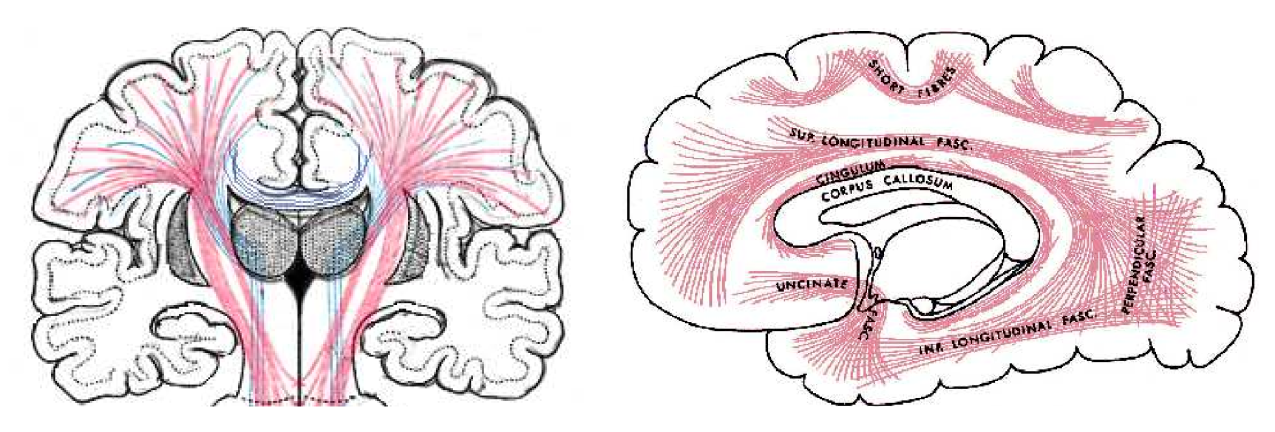
\includegraphics[width=\linewidth]{graysfibertracts}
	\caption{Example of human brain fiber tracts viewed from the front (coronal) and from the left (sagittal).  This image was derived from anatomical atlas diagrams in Gray's Anatomy \cite{odonnel06}.}
\end{figure}

Diffusion Tensor Imaging (DTI or DTMRI) is a recently developed Magnetic Resonance (MR) technique that reveals information about the layout of nerve fiber bundles in the brain.  Since nerve fiber bundles serve as interconnects between different neurological processing regions, information about these structures is crucial to a more complete understanding of the brain and the diseases which affect it.

Nerve tissue in the brain can be divided into gray and white matter.  Gray matter can be found throughout the brain but is concentrated on the cortical surface as well as in structures deep within the brain such as the thalamus.  The defining characteristic of gray matter is its lack of myelinated axons.  In contrast white matter is white in color because it has an abundance of myelinated axons.  Myelin consists mostly of lipids and gives white matter its color.  Bundles of these axons comprise white matter tracts. Figure \ref{fig:fibertracts} illustrates some prominent fiber tracts.

\section{Diffusion Tensor MRI Physics}

Typically, MRI is used to differentiate between different tissue types, such as gray and white matter.  This technique works by magnetically polarizing a particular slice of the brain.  A strong uniform magnetic field is applied to the entire brain causing the spins of most of the electrons to orient in the same direction.  Another magnetic field, this one nonuniform in space, polarizes the spins of the atoms in the brain differently depending on their location.  This gradient field is turned off and as the spins of the electrons reorient, or relax, back to the strong uniform field, they release a radio signal which is picked up by the receiving coil.  The frequency of these waves depends on their polarization which is dependent on their position in space.  The time needed for the spins to relax, known as the relaxation time, depends on the type of tissue the molecules exist in.  Using this data, an image can be constructed that differentiates between tissue types due to their characteristic relaxation time. Unfortunately, white matter appears homogeneous in anatomical MRI images and do not provide much information about the orientation of the white fiber tracts within each voxel.  Without this information it is not possible to reliably determine the connectivity between different regions of gray matter.  Diffusion Tensor Imaging is a recently developed MR technique which provides more information to characterize fiber tracts.

Diffusion Tensor Imaging (DTI) or DTMRI is an imaging technique that indirectly provides information about fiber tract orientation from the diffusion profile of water in the brain tissues. Diffusion in many parts of the brain occurs anisotropically, meaning its rate of diffusion is directionally dependent.  This anisotropy is believed to be caused by local physical constraints that impede diffusion.  The diffusion of water molecules, which are the predominant signal emitters in MR imaging, is believed to be constrained by the myelin that surrounds axons.  DTI images describe the diffusion profile of water within each voxel using a diffusion tensor.  These tensors can be thought of as ellipsoids with the eigenvectors describing the major and minor axes of the ellipsoid and the associated eigenvalues scaling these axes.  Isotropic diffusion profiles result in spherical ellipsoids while anisotropic diffusion profiles produce more eccentric ellipsoids.  The parameters which describe these tensors are obtained from Diffusion Weighted Images (DWI) of the same volume captured using at least six unique gradient directions and one reference image obtained in the absence of weighting gradients.

Each Diffusion Weighted Image (DWI) provides information about the magnitude of diffusion in one particular direction.  Diffusion Weighted imaging works similarly to anatomical MRI imaging but is additionally able to capture the Brownian diffusion of molecules during the imaging process.  Unlike anatomical MRI, an additional gradient magnetic field is applied in a choosen direction which then makes the resulting observations sensitive to the self diffusion of water in that direction. An MRI image obtained using these diffusion sensitizing gradients is referred to as a Diffusion Weighted Image or DWI.  Associated with each of these images is the direction of the magnetic field gradient used to polarize the molecules.  This information is necessary because different magnetic field gradients may result in significantly different DWI images due to the anisotropy of diffusion in certain regions of the brain.  Finally, this diffusion information can be used to estimate the parameters of a diffusion tensor which is then used to infer the orientation of fiber tracts in that voxel.

\section{Diffusion Tensor}
The diffusion tensor is a 3x3 symetric matrix which describes the distribution of diffusion within each voxel.  Because the matrix is positive definite, its eigenvalues are positive and represent the magnetude of diffusion in the direction of the eigenvector associated with that eigenvalue.

Because the tensor is sensitive to changes in the orientation of the object being scanned, clinical studies which attempt to compare different groups prefer to use properties of the tensor that are invariant to changes in orientation.  The most commonly used properties are the trace and the fractional anisotropy.  The trace the tensor is the sum of the diagonal components of the tensor and reprensents the average total diffusion.  A higher trace implies that there are few obstacles to water diffusion in that voxel.  The fraction anisotropy is given as
\begin{equation} \label{eq:tensormodel}
\sqrt{\frac{2*[(l\lambda_1-D_{av})^2 + (l\lambda_2-D_{av})^2 + (l\lambda_3-D_{av})^2]}
{2(\lambda_1^2+\lambda_2^2+\lambda_3^2)}}
\end{equation}

Fractional anisotropy is currently the most popular way to summarize the anisotropy of diffusion distribution expressed by the tensor.  FA ranges from 0 for isotropic diffusion to 1 for completely anisotropic diffusion.

%fill this in with related properties of the diffusion tensor
%various measures of anisotropy
%mathematic properties

\subsection{Visualization}
%[insert pictures]
%directionally coded images here
\begin{figure} \label{fig:visualization}
	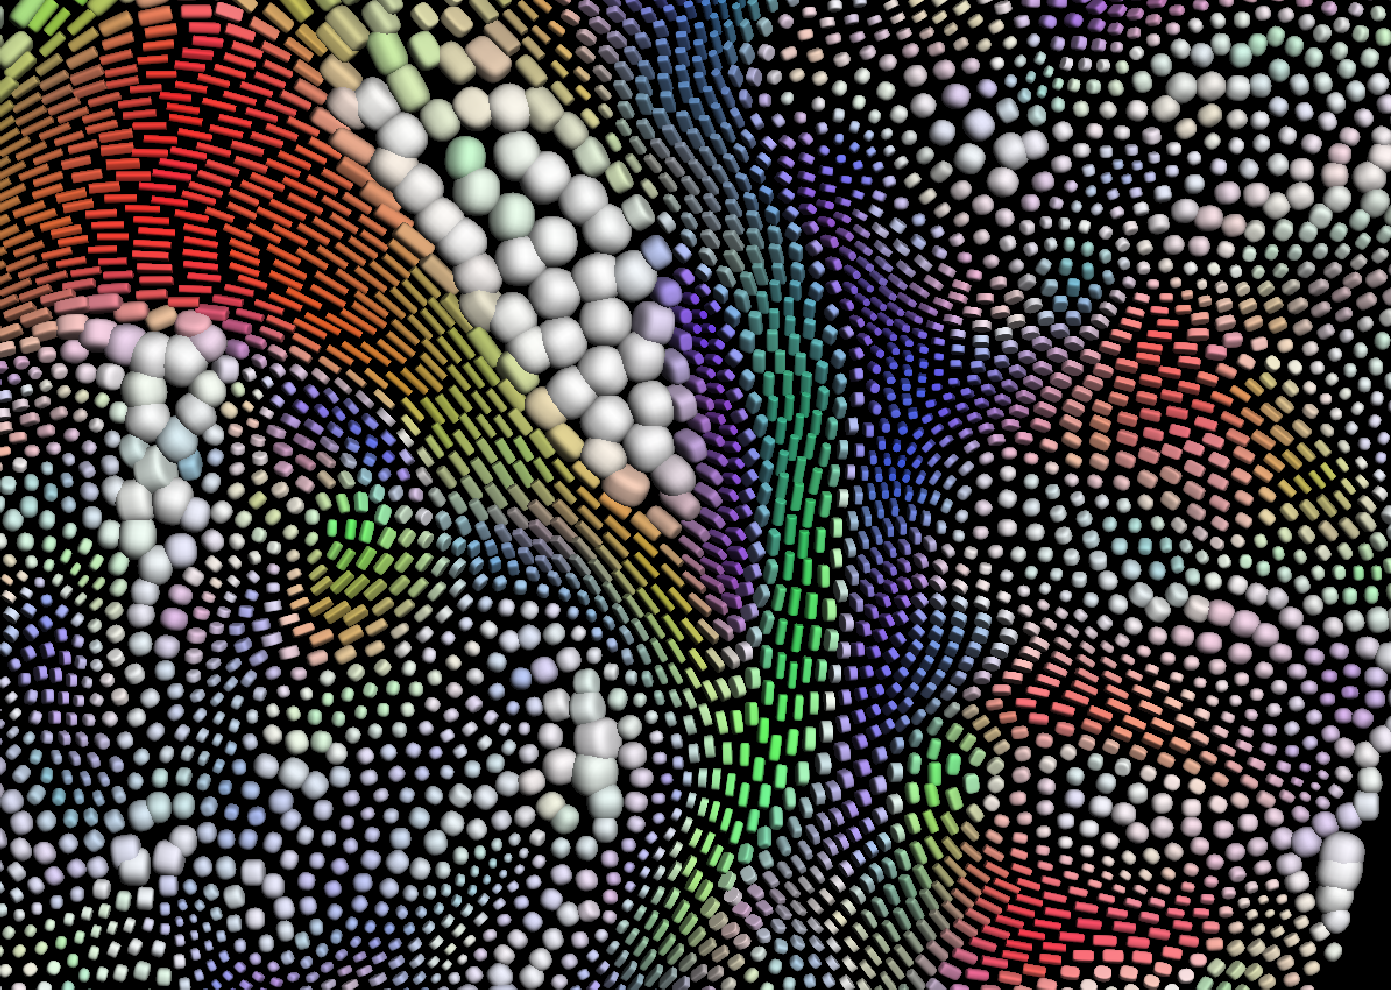
\includegraphics[width=0.5\linewidth]{packedglyphs}
	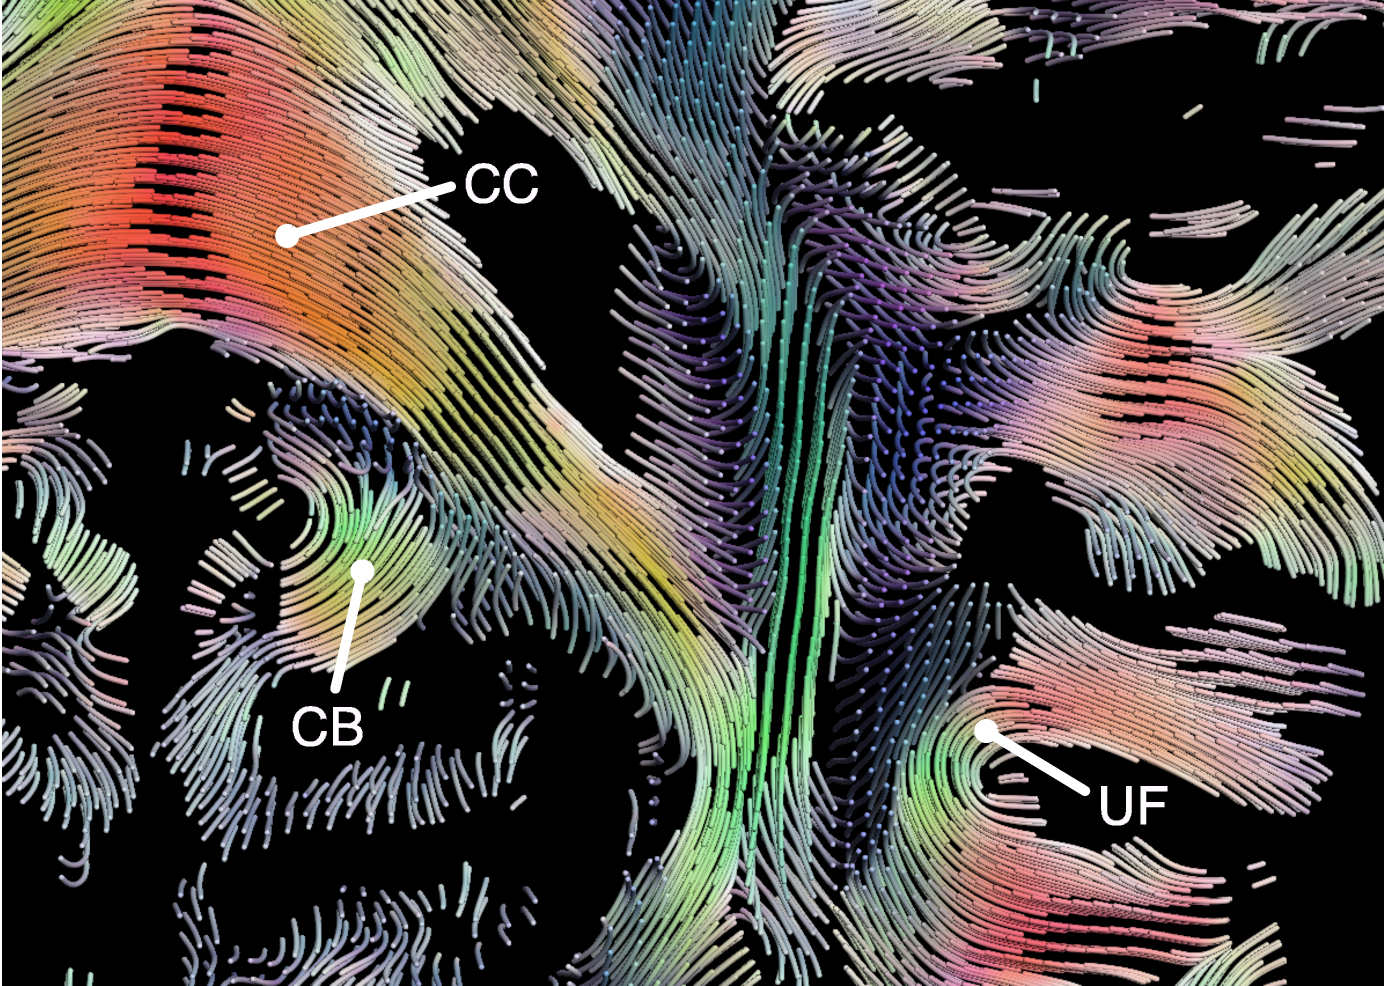
\includegraphics[width=0.5\linewidth]{tractography}
	\caption{DTI data visualization of major bundles using glyphs and streamlining tractography \cite{KindlmannTVCG2006}.  In the left image, DTI data is visualized using superquadric tensor glyphs. On the right, streamline tractography is performed on the same data.  The color in both images represent the estimated orientation of the fiber tract modulated by the degree of anisotropy in the data.  The color key is red is for left-right, blue for superior-inferior, green for anterior-posterior.  Regions that are white have low anisotropy while saturated regions exhibit highly anisotropic diffusion.}
\end{figure}


The two primary ways to visualize DTI data is through the use of glyphs and tractography.  Figure \ref{fig:visualization} demonstrates these two methods.  Glyphs are visual representations of the tensors at each voxel in one slice of DTI data.  Glyph visualization is good for understanding local, voxel-specific tensor data but is not as useful for interpreting inter-voxel patterns.  Tractography overcomes this limitation by inferring fiber tracts from regular patterns in the diffusion tensor image.

\section{Tractography}
%talk about as manny past works in DTI as possible
%name them by what the authors have called them
%Survey of White Matter Tractography
%Behrens
%Bootstrap
%Fast marching
%Stochastic Tractography
Tractography can be performed in a number of ways. One method is to draw tracts which follow the underlying tensor's major eigenvector, the direction of greatest diffusion.  These methods are known as streamlining methods and have been investigated by a number of researchers \cite{behrensMRM03}.  Streamlining approaches attempt to generate tracts by tracing the principle diffusion direction predicted by the diffusion tensor.  Although this method successfully generates tracts in most parts of the brain, it is difficult to believe these results because there is no information about the confidence in the generated tracts.  The uncertainty in tract location and orientation stem from noise, distortions, insufficient resolution, and partial volume effects.  Partial volume effects are caused by crossing fibers within a single voxel.  Such crossings contribute additional uncertainty due to the lack of a model which sufficiently describes the effect of crossing fibers on the MR signal.  Additionally, since streamlining methods trace the principle diffusion direction, they are only able to trace fibers in regions with relatively high anisotropy.  Regions with reduced anisotropy increase uncertainty about the fiber orientation.  Important gray matter regions contain areas of reduced anisotropy.  Since streamlining is unable to generate tracts in gray matter, it is difficult to estimate the connectivity of these important regions of neural processing with other parts of the brain.  Probabilistic tractography overcomes these shortcomings by explicitly modeling the uncertainty in the local fiber orientation.

\chapter{Stochastic White Matter Tractography}
Stochastic tractography, sometimes known as probabilistic tractography, differs from streamlining methods in that it takes into account the uncertainty in fiber orientation when estimating the fiber tracts.  Probabilistic methods perform tractography under a probabilistic framework which explicitly models the uncertainty in the generated tracts.  Since the local uncertainty of the fiber orientation is modeled, probabilistic methods can generate tracts in regions of low anisotropy.  In streamlining methods, the tractography algorithm is arbitrarily prohibited from generating tracts in regions of low anisotropy because that section of the generated tract would be highly uncertain.  In contrast, probabilistic methods are able to generate tracts which momentarily pass through regions of low anisotropy because they able to integrate this local fiber orientation uncertainty into the uncertainty of the entire tract. As a result a probabilistic method, unlike streamlining methods, can perform tractography in low diffusion anisotropic areas such as gray matter \cite{behrensMRM03}.

\section{Modeling Approaches}
Probabilistic methods must infer the probability density of the fiber orientation from DWI data.  These methods can be classified as either nonparametric or parametric.  In nonparametric approaches, the probability density is approximated by repeated empirical sampling of the fiber orientation distribution.  Nonparametric methods make no assumptions about the underlying probability distribution, but as a consequence require more data to create a good approximation.  In contrast, parametric methods make assumptions about the underlying probability density, which greatly reduces the number of empirical samples needed to create an approximate distribution. The assumptions are captured in a model which describe the assumed relationships between the data and the fiber orientation distribution.  As a result, the assumptions made in parametric methods greatly influence the approximated probability distribution.

The bootstrap method is a nonparametric procedure which can provide confidence information regarding tracts generated using any streamlining tractography algorithm.  The method requires obtaining redundant sets of DWI data.  Jones et al. \cite{derek} obtains nine redundant sets of DWI volumes to perform the bootstrap method.  Random combinations of DWI volumes are sampled from this pool to generate a large number of complete mixed DWI sets known as bootstraps.  Using a streamlining tractography algorithm, deterministic tractography is performed on each bootstrap set at the same starting, or seed location.  A visitation percentage is then calculated for each voxel in the volume indicating the percentage of sample sets which generated a tract that passed through that particular voxel.

Parametric tractography methods use a probabilistic model to relate the observed data to a probability density function of the underlying fiber orientation.  The fiber orientation model constitutes a local model which is applied to every voxel.  The methods use the local model of orientation to construct a global model of connectivity between regions.  A streamline-like tractography method is then used to generate tracts by randomly sampling fiber directions from the fiber orientation PDF at each voxel as calculated by the local model.  The path can now be considered a probabilistic process since it is generated from repeated samplings of a probability density function.  Many realizations of the path are generated from a single seed point.  These paths are then used to generate a connectivity probability map.  In accordance with the global model, the probability that region $A$ is connected to region $B$ can then be found by calculating the fraction of paths that pass through region $B$ originating from $A$.

%need to reconsider this comparison
Parametric and nonparametric methods have different strengths and weaknesses.  The strength of nonparametric methods is that the probability density is obtained empirically, without the need for unproven models.  However, nonparametric methods require a large amount of DWI data and obtaining the necessary data currently requires impractically long scan times \cite{derek}.  Therefore, unless scanning technology improves to reduce these scan times, parametric methods are most practical for clinical studies.

Behrens's parametric approach pioneered the field of probabilistic tractography\cite{behrensMRM03}. Behrens's model makes the simplifying assumption that only a single fiber passes through a voxel.  Deviations from this simple model due to crossing fibers is captured as uncertainty in the fiber orientation.  In this model a voxel is described as two compartments whose net diffusion profile is the sum of a small anisotropic diffusion component that occurs in and around the fiber and a larger isotropic diffusion component outside of the fiber.\cite{behrensMRM03}.  The fiber orientation distribution is analytically intractable and Behrens overcomes this issue by computing the PDF using Markov Chain Monte Carlo (MCMC) techniques.  MCMC is a method to numerically integrate an analytically intractable integral.  

Friman's approach is similar but suggests optimizations to Behrens's approach \cite{frimanTMI06}.  In contrast with Behrens's work, the model used by Friman is derived from the well known tensor model of diffusion.  The tensor model of diffusion attempts describes diffusion in each voxel using a symmetric tensor.  The Friman model assumes the two smallest eigenvectors of diffusion tensor are equal, constraining the shape of the diffusion tensor to a "cigar-like" shape. 

%need to add in a bit about how they are different in the way they sample the PDF
The parametric approaches developed by Behrens and Friman are conceptually similar but differ mainly in their methods of arriving at the probability density function of the fiber orientation.  Their methods differ both in the model they use to describe the relationship between fiber orientation and the DWI data as well as the method they use to sample the fiber orientation probability density function resulting from the choice of model.  Whereas Behrens's directly models the fiber orientation, Friman's model is concerned with the diffusion profile and infers the fiber orientation from this profile.  Although Behrens's two-compartment model may be more conceptually sound, the advantage of using Friman's "constrained model" is its mathematical tractability.  The constrained model is able to fit every voxel within a matter of seconds whereas Behrens model takes a couple of hours \cite{frimanTMI06}.  Additionally Friman avoids using MCMC techniques by assuming that parameters other than the principle diffusion direction are constant within each voxel.  Friman further demonstrates that these mathematical simplifications have little effect on the resulting tractography.  This project will implement Friman's approach to probabilistic tractography.

\section{Probabilistic Tractography Theory}

Friman's probabilistic tractography algorithm \cite{frimanTMI06} operates at two levels.  At the local level, he presents a constrained model of diffusion that is describes the relationship between the DWI data and the likelihood of a fiber tract producing that data.  At a more global level, fiber tract orientation distributions are sampled across many voxels to infer the probability that two regions in the brain are connected by a fiber tract.  This distinct division is also found in Behrens's original work \cite{behrensMRM03} on probabilistic tractography.

%[most have been voxel based,
% ROI studies, select a subset of voxels belonging to a particular fiber bundle of interest]
%[ROI studies sometimes select voxels in only one slice, which may not capture the information presented by the entire fiber tract...]
\section{Tractography in Clinical Studies}
The fiber tract information provided by DTI has been valuable for neurological studies.  For instance, clinical DTI studies have demonstrated differences in diffusion anisotropy within fiber tracts in Schizophrenia patients compared with healthy patients \cite{kubickiBiologPsych03},\cite{kubickiNI05}.  This is significant because it has been suspected that Schizophrenia may be associated with structural abnormalities in fiber tracts.  However, many of these studies are limited to comparing tensor information on a per voxel basis inside a region of interest on a DTI slice.  Although this analysis is straightforward, it is limited in the information it can provide and may actually introduce errors.  It is difficult to determine if observing a slice of a fiber bundle in one patient corresponds with observing the same slice in another patient.  Additionally such local studies do not compare the structure of the entire fiber tract which exists in three dimensions.  Comparing the entire fiber tract will alleviate the above problems.  A rigorous comparison of these tracts will require confidence information about the estimated tracts.  Unlike streamlining tractography methods, probabilistic tractography provides the confidence information and promises to enable clinical studies of holistic fiber tract differences.
